\documentclass{article}
\usepackage[utf8]{inputenc}
\usepackage[brazil]{babel}
\usepackage{epsfig}
\usepackage{fancyhdr}
\usepackage{indentfirst} %In­dent first para­graph af­ter sec­tion header
\usepackage{titlesec}
\usepackage{amsmath}
\usepackage{amsthm}

\pagestyle{empty}

\headheight 40mm      %
\oddsidemargin 2.0mm  %
\evensidemargin 2.0mm %
\topmargin -40mm      %
\textheight 250mm     %
\textwidth 160mm      %
%
\newcounter{execs}
\setcounter{execs}{0}
\newcommand{\exec}[0]{\addtocounter{execs}{1}\item[\textbf{\arabic{execs}.}]}

\fancypagestyle{first}
{
\pagestyle{fancy}
}
%%%%%%%%%%%%%%%%%%%%%%%%%%%%%%%%%%%%%%%%%%%%%%%%%%%%%%%%
%%%%%%%%%%%%%%%%%%%%%%%%%%%%%%%%%%%%%%%%%%%%%%%%%%%%%%%%
% PLEASE, EDIT THIS!
\fancyhead[LO]{\small $5^a$ Lista \\ 
                DCC008 - Cálculo Numérico  \\
                \textbf{Entrega: 11 de Novembro de 2018} }

\fancyhead[RO]{\small Universidade Federal de Juiz de Fora - UFJF \\ 
                Departamento de Ciência da Computação \\
               \textit{Nome: Thiago de Almeida}\\
               \textit{Nome: Aluno 2}}


\begin{document}
\thispagestyle{first}
%    \noindent \textbf{Obs1.:}  Escolha um ou mais métodos de interpolação dado em aula para resolver os problemas abaixo.
%    
%    \noindent \textbf{Obs2.:}  Discuta os resultados.

\begin{itemize}

\exec O arquivo ``dados.txt'' contém os dados históricos referentes a cotação diária das ações da empresa Petrobras (PETR4) nos últimos 2 anos, que são negociadas na bolsa de valores de São Paulo (BOVESPA). 

\begin{itemize}

\item[a)] Apresente gráficos comparando os dados do arquivo ``dados.txt'' com as curvas ajustadas pelo método de mínimos quadrados para diferentes ordens polinomiais ($P_n(x)$, $n=1,3,5,10,15,20,50,100$).

\item[b)] Definindo como $x$ a primeira coluna e $y$ a segunda coluna do arquivo ``dados.txt'', calcule, para todos as ordens polinomiais do item (a), o coeficiente de determinação $r$ que pode ser calculado como:
$$
r^2= 1 - \dfrac{\displaystyle \sum_{i=1}^{k} \left(y_i-P_n(x_i) \right)^2}{\displaystyle \sum_{i=1}^{k} y_i^2 - \dfrac{1}{k} \left(\sum_{i=1}^{k} y_i \right)^2 }
$$
onde $k$ denota a quantidade de dados do arquivo ``dados.txt''. Monte uma tabela apresentando os resultados do coeficiente de determinação $r$ em porcentagem ($r*100$).

\item[c)] A partir dos resultados da letra (b), utilize a curva que melhor se adapte aos dados fornecidos para projetar os preços da ação para os próximos 100 dias e apresente um gráfico com este resultado. 

\end{itemize}

\end{itemize}

Analisando os dados de cotação diária da empresa PETR4 nos ultimos 2 anos através do método dos minimos quadrados. Obtem-se os seguintes resultados:

\newpage
\begin{figure}[!htb]
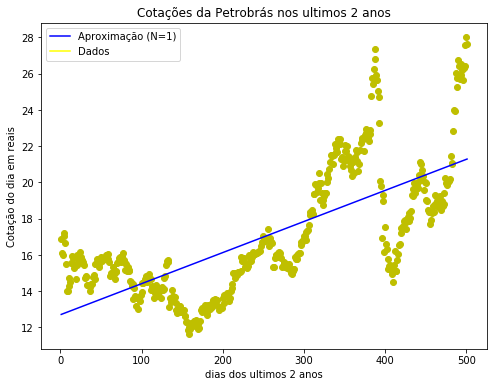
\includegraphics [width=6cm,height=6cm]{G1.png}
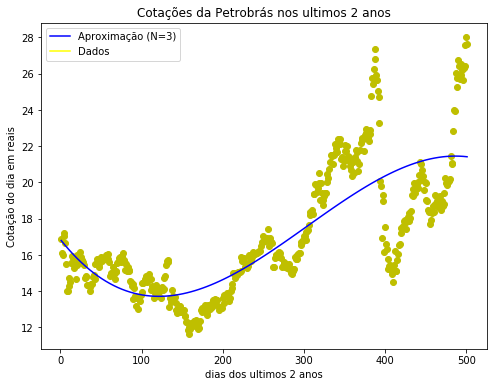
\includegraphics [width=6cm,height=6cm]{G3.png}
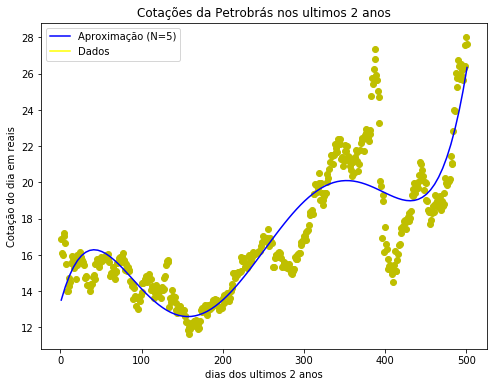
\includegraphics [width=6cm,height=6cm]{G5.png}
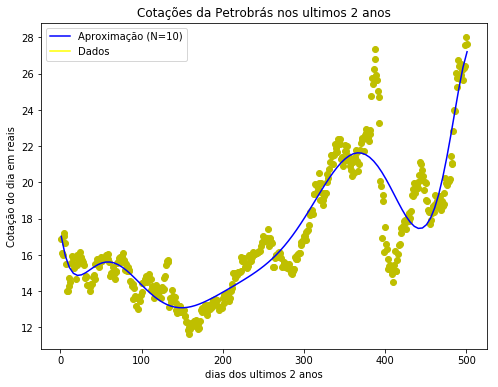
\includegraphics [width=6cm,height=6cm]{G10.png}
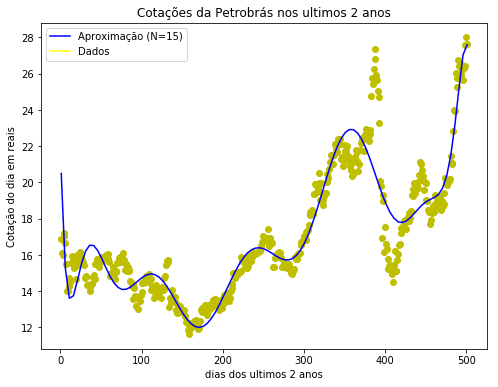
\includegraphics [width=6cm,height=6cm]{G15.png}
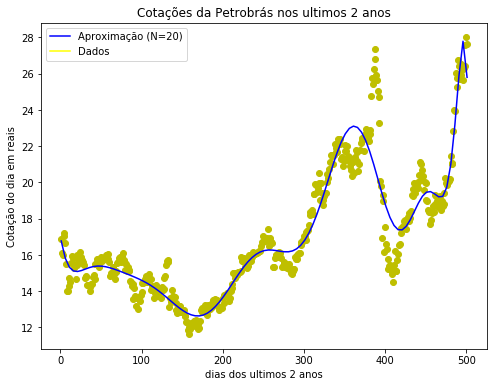
\includegraphics [width=6cm,height=6cm]{G20.png}
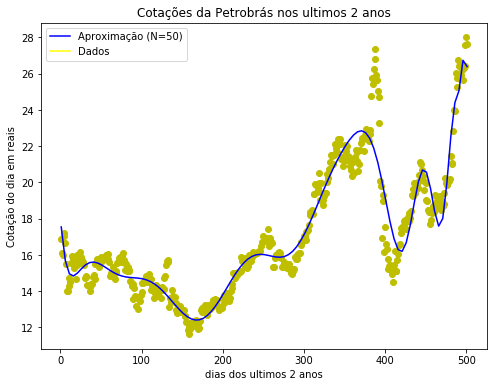
\includegraphics [width=6cm,height=6cm]{G50.png}
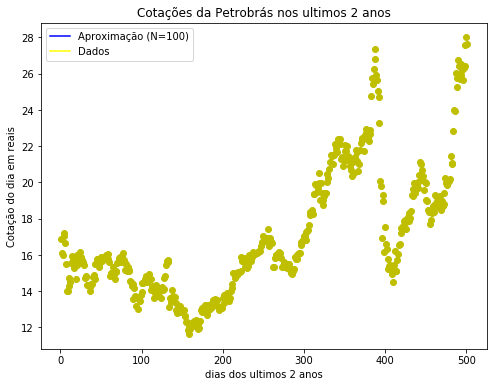
\includegraphics [width=6cm,height=6cm]{G100.png}
\end{figure}

\newpage

Observando os valores, o método funciona bem para as ordens polinomiais até a ordem $n <= 56$, após esse resultado o valor aproximado não consegue ser capitado pela máquina usando a precisão de float64.

\begin{figure}[!htb]
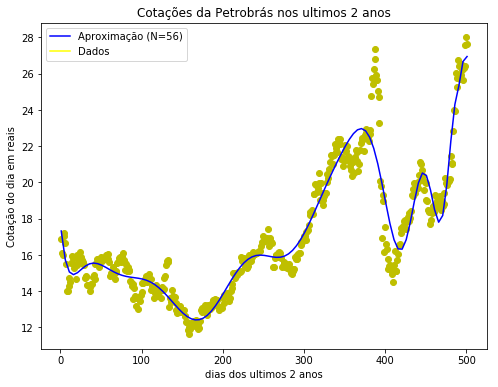
\includegraphics [width=8cm,height=8cm]{G56.png}
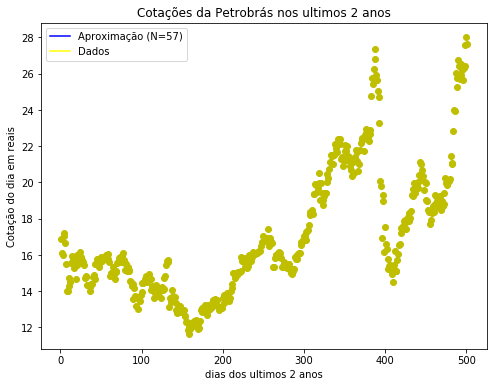
\includegraphics [width=8cm,height=8cm]{G57.png}
\end{figure}


\text Definindo as colunas x e y para o método polinomial do item (a), o coeficiente r que pode ser calculado e expresso em porcetagem é:
\begin{table}[h]
\centering
  \begin{tabular}{l|l|lll}
    $Ordem$ $n$ & $Coeficiente$ $r$ & $Coeficiente$ $r$ $em$ $porcetagem$ $(\%)$\\
    \hline
    1 & 0.7109284708160442+0j & 71.092\\
    
    3 & 0.7910095119409309+0j & 79.100\\
    
    5 & 0.8750227594557071+0j & 87.502 \\
    
    10 & 0.9132363940671044+0j & 91.323\\
    
    15 & 0.9353002361833165+0j  & 93.530\\
    
    20 & 0.9401289596912272+0j & 94.012\\
    
    50 & 0.9541317215035551+0j & 95.413\\
    
    100 & nan+nanj & nan\\
    \hline
  \end{tabular}
  \caption{coeficiente r em porcetagem}
\end{table}

\text Todos os testes acima foram realizados 
\end{document}
